%-----------------------------------------------------------------------------------
%	PACKAGES AND OTHER DOCUMENT CONFIGURATIONS
%----------------------------------------------------------------------------------

\documentclass[11pt]{article}

\usepackage[top=2cm, bottom=3cm, left=2cm, right=2cm]{geometry}
\setlength{\parskip}{1em}
\setlength{\parindent}{4em}
\linespread{1.25}

\newcommand{\Var}{\mathrm{Var}}

\newcommand{\Cov}{\mathrm{Cov}}

\newcommand{\plim}{\rightarrow_{p}}

\usepackage{apacite}

\usepackage{amsmath, amsfonts}
\usepackage{graphicx}
\usepackage{pdfpages}
\usepackage{bm}
\usepackage{listings}
\usepackage{multirow,array}
\usepackage{enumerate}
\usepackage{bbm}
\usepackage{subfig}


\usepackage[latin1]{inputenc}

\usepackage{amssymb}

\usepackage{mathrsfs}
\usepackage{float}
\usepackage{booktabs}
\usepackage{color}
\usepackage{rotating}
\usepackage{amsthm}
\usepackage{multirow,array}
\usepackage{caption}
\usepackage{url}



\DeclareMathOperator*{\argmax}{arg\,max}
\DeclareMathOperator*{\argmin}{arg\,min}



% Expectation symbol
\newcommand{\E}{\mathrm{E}}
\newcommand{\V}{\mathrm{V}}
\newcommand{\N}{\mathcal{N}}
\newcommand{\R}{\mathbb{R}} 

%----------------------------------------------------------------------------------
%	TITLE AND AUTHOR(S)
%----------------------------------------------------------------------------------

\title{Marijuana legalization and alcohol consumption:\\
	Labor Rough Draft} % The article title

\author{Nathan Mather} % The article author(s) 

\date{\today} % An optional date to appear under the author(s)

\renewcommand{\contentsname}{Table of Contents}
%----------------------------------------------------------------------------------
\begin{document}
	
	
%------------------------------------------------------------------------------
%	TABLE OF CONTENTS
%------------------------------------------------------------------------------
\maketitle % Print the title/author/date block

\setcounter{tocdepth}{3} % Set the depth of the table of contents to show sections and subsections only

\tableofcontents % Print the table of contents

%------------------------------------------------------------------------------
% Introduction 
%------------------------------------------------------------------------------
\section{Introduction}
\subsection{Motivation}

In 2012 Colorado and Washington voted to legalize recreational marijuana in a bold move that defied federal laws.  While there was some uncertainty around how the federal government would react and if recreational dispensaries would be allowed to operate. In terms of bucking federal law, offering legal recreational marijuana, and collected tax revenue, this experiment proved to be a success. In 2014, the first year recreation dispensaries opened, Colorado had \$683,523,739 in sales and \$67,594,323 collected in taxes \cite{Colorado_marijuana_sales}. California , D.C., Maine, Massachusetts, Nevada, Oregon, Vermont, Washington, and Michigan have all followed suit since and enacted some form of legal recreation marijuana. These policies have been a success in terms of implementing their stated goals, but what has the impact of readily accessible marijuana been on public health? \par

There are a variety of factors that influence this question, but one key component is how easier access to marijuana will affect the consumption alcohol. While there is much debate about the extent to which marijuana causes public harm, there is little doubt that increased consumption, all else equal, will come with some costs. While the impact of marijuana on individual health is still in need of additional research, Marijuana can impair motor skills and can lead to traffic fatalities \cite{webmd_mj}. Of course, all else is not equal.  Despite potential harmful effects, if marijuana acts a substitute for alcohol, which may have more serious negative public health impacts, the general equilibrium effect may be a public health win. If Marijuana is a compliment to alcohol, however, then legalization of marijuana may increase the negative impacts of alcohol. \par


There are many concerns unrelated to public health that come into play in the normative discussion around marijuana legalization. I do not expect that the relationship between alcohol and marijuana to end this discussion. However, understanding all the implications of legalization will give policy makers a clearer picture of the costs and benefits involved and may help guide specific policy to ensure a smooth rollout of marijuana legalization policies.




\subsection{My contribution to Literature}

The existing literature on the relationship between recreational marijuana legalization and alcohol consumption, that I can find, is fairly limited. Most of the published work either considers the relationship between marijuana and alcohol through the lens of medical marijuana or does not focus on the relationship recreational marijuana has specifically on alcohol.\par 


A paper by Baggio, Chong, and Kwon addresses the substitutability of marijuana and alcohol by using retail scanner data and variation in medical marijuana laws. They use a fixed effects model of counties across the united states over time. Their variable of interest is if the county has medical marijuana or not. They find that Counties located in MML states reduced monthly alcohol sales by 15 percent" \cite{baggio_chong_kwon_2018}. I use a similar approach to examine the impact of recreational marijuana. I also use the retail scanner data, but also consider the geographic distribution of marijuana retailers within a state over time. While legalization increases access it's effects are likely different if a retail location is readily available. \par


The above paper and the approach I have taken are light on theory. However, a paper by Miller and Seo that analyzes the complementarity of marijuana and alcohol  the context of tax revenues and uses a more theory driven approach. To set up this problem they use a multistage budgeting approach. The top stage is substances. The second stage is Marijuana, alcohol, or tobacco. Finally, the third stage is which types of each product to consume, beer or wine for example. They estimate their model using the Nielson Scanner data and data on sales and prices of marijuana directly from Oregon. To account for endogeneity, they use wages and county and time fixed effects as an instrument for prices as well as wholesale prices and taxes.  They cast doubt on the validity of using surrounding states as a control since Oregon saw significant alcohol price changes around the time of the change. They instead use price changes within Oregon after legalization along with this model to tease out this relationship \cite{miller_seo_2018}. \par


While their approach incorporates prices and does not rely on comparing states that differ in potentially unaccounted for ways, there are other issues with their specification. Most importantly their estimation strategy requires estimating the actual quantity of marijuana consumed. They actually point out themselves that prior to legalization an estimated 85 to 225 metric tons of marijuana was sold in Washington while only 29 metric tons was sold after legalization \cite[p.~13]{ miller_seo_2018}.  While they try to explain away the difference with varying THC concentrations, it is not a convincing argument for this dramatic of a difference. Additionally, we may actually expect new customers from out of state coming into Washington and inflating sales. Making the 29 ton number see especially small. \par


Miller and Seo also run into problems because they need prices for their equations, but prices are endogenous to the demand for products. They attempt to solve this problem by instrumenting for prices. By using the shock of legalization and subsequent opening of retail locations I avoid this problem. While states that legalize marijuana likely have more demand for drugs in general, including alcohol, I do not expect it was a sudden shock to demand right before legalization that led to the policy. Rather, it was pressure over time from existing support. These long-term differences can be captured with fixed effect and should not bias direct estimates of the impact of legalization. By considering a policy specific shock, however, I lose the level of precision that allows them to estimate an actual cross price elasticity. Instead, I get a coefficient based on policy specific parameters like the number of dispensaries. 





\subsection{Outline}






I have considered multiple analytical approaches and data sources to address the impact of legalization and readily accessible marijuana on alcohol consumption. the remainder of the paper will proceed as follows. First, I will discuss the theoretical approach I am using to answer this question. Specifically, I explain why I think the event of legalization and opening of dispensaries has sound theoretical footing to address this question. Next, I will discuss the data sources I use. These include the CDC's Behavioral Risk Factor Surveillance System survey, the Nielson Scanner data, and geographic data on dispensary locations. After reviewing the data, I will walk through the analytical methods employ and discuss the results. Finally, I will discuss the shortcomings and areas of improvement for my paper and how I hope to address these moving forward. 

%------------------------------------------------------------------------------
% Theoretical Approach
%------------------------------------------------------------------------------

\section{Theoretical Approach}

I aim to determine the effect of marijuana legalization and readily accessible recreational marijuana on alcohol consumption. This policy specific question can also be stated using the basic theory of compliments and substitutes. That is, are marijuana and alcohol compliments or substitutes.  
To answer this question  I rely on the assumption that legalization and recreational dispensaries lower the cost of consuming marijuana. This assumption comes from two aspects of recreational marijuana legalization and basic theory. The first is that legalization directly lowers the cost of consuming marijuana by eliminating the risk of legal repercussions. Let the expected cost of purchasing and consuming illicit marijuana be C. If we are considering legalization alone then C is simply the costs or expected legal risks associated with purchasing an illegal substance. If we are considering legalization along with readily accessible retail marijuana dispensaries than C could also include the inconveniences of purchasing marijuana from an individual rather than a retail location with laws regulating trade. 

With this in mind, prior to legalization, consumers are effectively paying $P_B + C$, the black-market price plus the cost of illegal activity. Legalization will increase the marginal benefit of marijuana consumption by C. On its own, this would actually lead to an increase in the demand for marijuana and thus an increase in the market price and quantity; however, as figure 1 shows, the old effective price $ P_B + C$ is still greater than the new market price $P_E$ (which is also the effective price in the absence of legal repercussions). This leads to a reduction in the real price for consumers from $ P_B + C$ to $P_E$. If marijuana and alcohol are substitutes, this should decrease demand for alcohol even though the list price of marijuana is increasing.\par
\begin{center}
	\centering
	
	\textbf{Figure 1}\par\medskip
	
	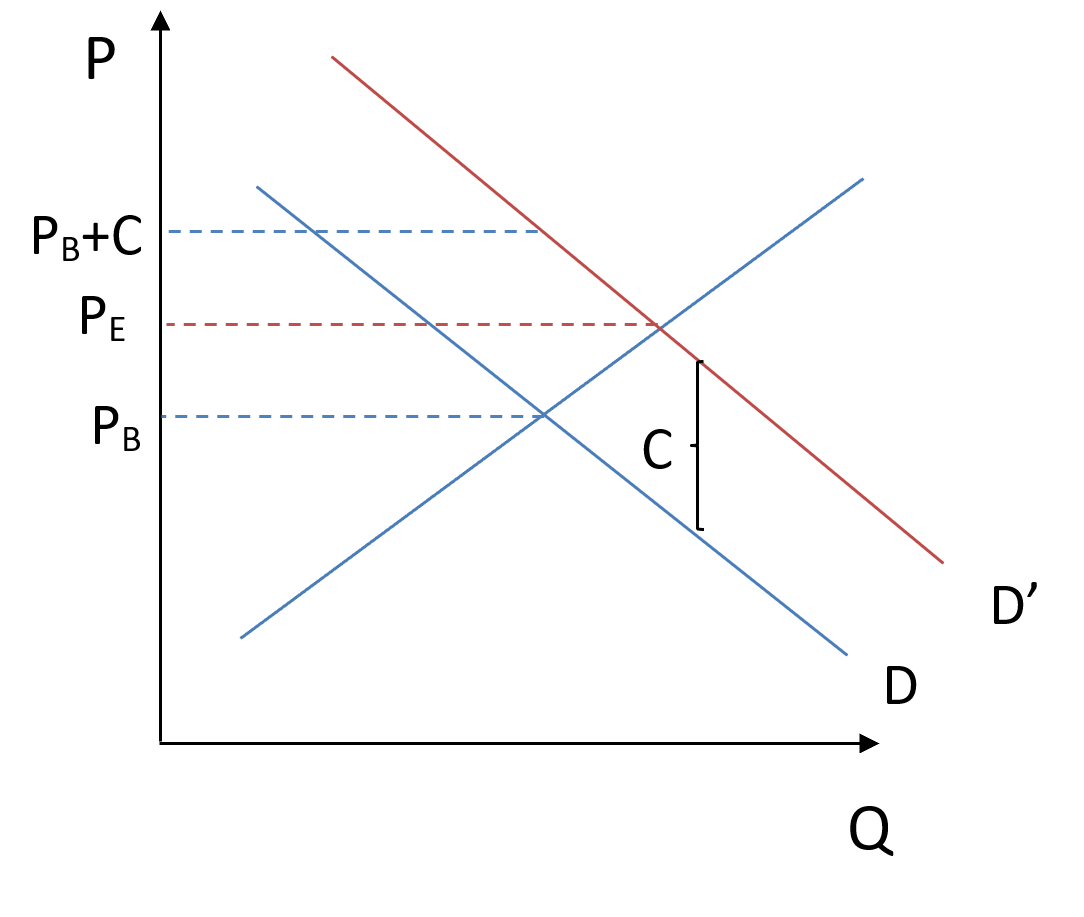
\includegraphics[width=.5\linewidth]{legal_dside.png}
	
\end{center}


In addition to the demand effect, legalization will also lower the marginal cost of production. Lower marginal costs for producers results in a basic shift to the right of the supply curve. As legal action against growers and suppliers is generally more harsh than consuming small amounts, I suspect the magnitude of this shift will be large relative to the demand shift. Additionally, by allowing recreational dispensaries and formal businesses in marijuana production and distribution, economies of scale will further increase supply. This rightward shift in the supply curve also works to lower the price of marijuana to consumers. \par

One objection that could be made to this claim is that price controls and burdensome regulation on the legalized production and sale may lead to a higher price for regulated marijuana than the prior price of black-market marijuana. It is important to remember, however, that the black market is still an option for producers and consumers. Taken to the extreme, regulation may be so burdensome that no dispensaries open and legalization does not shift supply to the right at all. In this case, however, the observed market price may be higher for consumers, but, as figure one shows, the effective price is still lower as the risk of legal repercussions has fallen. \par
With the seemingly safe assumption that legalization of recreational marijuana will lower the effective price paid by consumers, I can appeal to the basic theory of compliments and substitutes. If marijuana and alcohol are compliments, we should see alcohol consumption rise as a result of the policy shocks. If they are substitutes, we should see alcohol consumption fall.\par




%------------------------------------------------------------------------------
% Data
%------------------------------------------------------------------------------

\section{Data}

In order to measure alcohol use I first turned to the state-based Behavioral Risk Factor Surveillance System (BRFSS) put out by the Centers for Disease Control and Prevention (CDC). it is "a cross-sectional telephone survey that state health departments conduct monthly over landline telephones and cellular telephones with a standardized questionnaire and technical and methodologic assistance from CDC" \cite{BRFSS_homepage}.The survey has a sample size of around 500,000 a year. The survey includes two questions that together give average weekly drinks per week. These include: how many days per week or per month did you have at least one drink of any alcoholic beverage such as beer, and how many drinks do you usually have when you drink. \par


I was initially very optimistic about this data. This survey has the advantage covering all alcohol consumption for the individuals surveyed as well has having a large sample size. The survey also provides a rich set of covariates. In theory, this could offer a detailed look at alcohol use, but I have uncovered a number of issues. The biggest of which is measurement error. Alcohol consumption is a sensitive topic for many. Not only is there the possibility that some people intentionally misrepresent their consumption, people may not even be able to honestly recount their use. While I expected people to constantly lie downwards and underreport their drinking habits, there are a number of extremely large outliers that must either be intentional misrepresentation or possibly entry errors. For example, there are entries of averaging over 70 drinks a day for 30 days out of the month. If the measurement error is random it shouldn't systematically bias the results, since alcohol use is the dependent variable, but it may make it hard to detect a statistically significant result. To deal with this I have truncated the data at the 99th percentile. This potentially biases the results, but it's also removing some false data that would also bias the results; so, I think it is a reasonable strategy. The data also only gives me the respondents state of residence and is not a panel. This means I can only include state fixed effects and the only variation in marijuana policies and access will occur at the state level. \par

While analyzing the BRFSS data is instructive, the issues uncovered warrant including an additional alcohol use measure and alternative analysis.  I also use Alcohol sales data from the Nielson Retail Scanner Data . Nielson collects alcohol sales directly from retailers on a weekly basis. Measuring alcohol use in this way does have some drawbacks compared to the BRFSS survey. Alcohol sales in bars and restaurants are completely left out of the sample. Additionally, we are limited to the retail chains that accept the survey. That being said, there is extensive coverage. The Figure in Appendix A shows the number of counties with sales data per month in unbalanced panel going from 2011 to 2016. I drop any counties that are in less than ten months of data because I use county fixed effects in the model using this data. I only use data going back to 2011 even though the scanner data goes back to 2006 because recreational marijuana does not take place in any state until 2014 and I wanted to limit the amount of pre-treatment data to a more reasonable level. This was done in an ad-hoc way because the fixed effect model should account for pre and post time trends. The Data ends in August of 2016 because in September of 2016 the first recreational marijuana dispensaries opened in Oregon. I only have dispensary data for Washington and Colorado, so I cut the time series 3 month short of the full Nielson sample. \par

My dispensary data comes from the Washington State Liquor \& Cannabis Board and the Colorado Department of Revenue Enforcement Division. The data sources give me a monthly snapshot of every licensed retailer and their address. Using the Texas A\&M Geocoding services I convert these address into latitude and longitude coordinates \cite{tamu}.To determine what county each dispensary is in as well as their distance to other counties I use the Cartographic County Shape files from the United States Census Bureau \cite{branch_2018}. Figures 1 and 2 show the evolution of marijuana dispensaries in Colorado and Washington over time. We can see that the number of dispensaries stabilized more quickly in Colorado while Washington has had a slower expansion. \par


\begin{figure}[H]
	\centering
		\LARGE{\textbf{Figure 1}}
	\subfloat{
		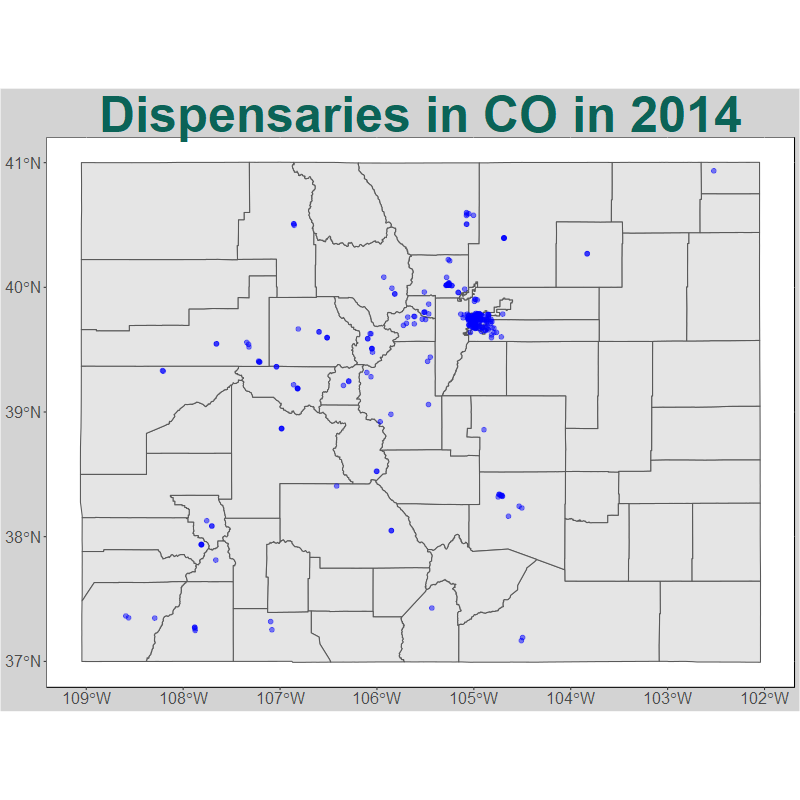
\includegraphics[width=.5\linewidth]{point_map_CO_2014.png}
	}
	\subfloat{
		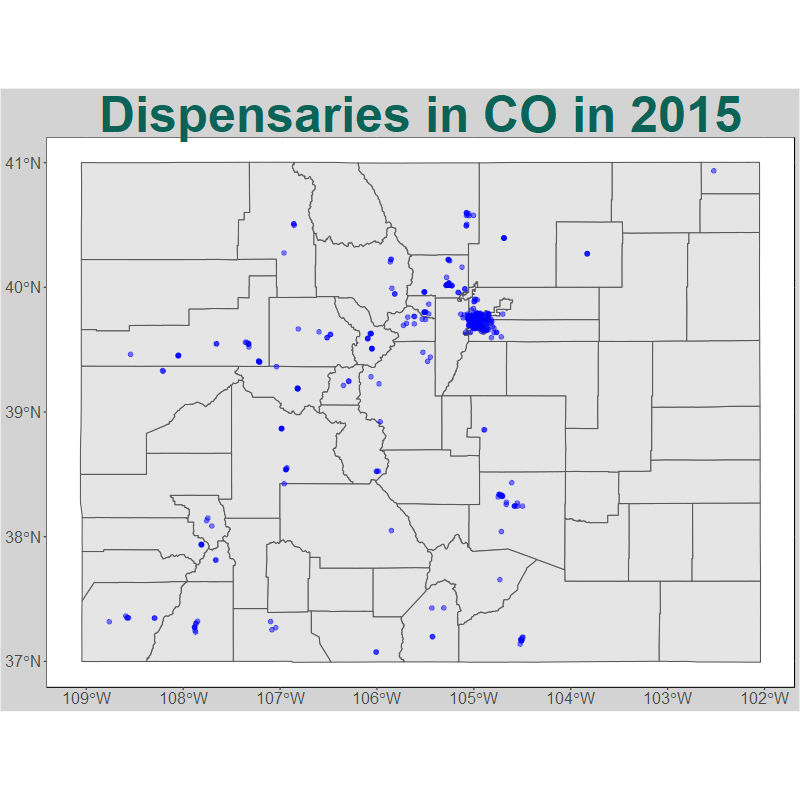
\includegraphics[width=.5\linewidth]{point_map_CO_2015.png}
	}
\newline
	\subfloat{
		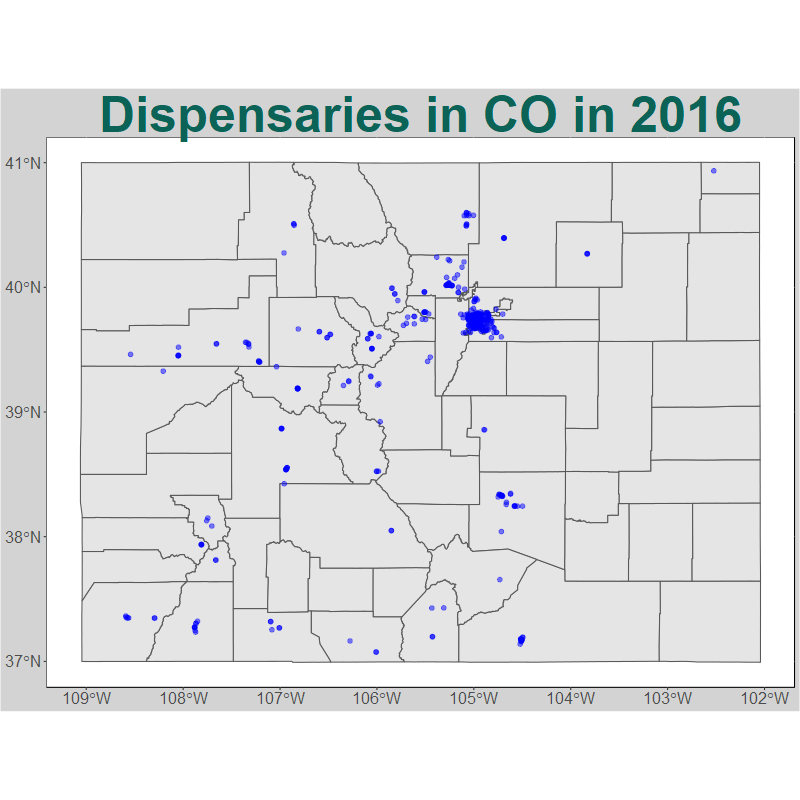
\includegraphics[width=.5\linewidth]{point_map_CO_2016.png}
	}
-
\end{figure}

\begin{figure}[H]
	\centering
	\LARGE{\textbf{Figure 2}}
	\subfloat{
		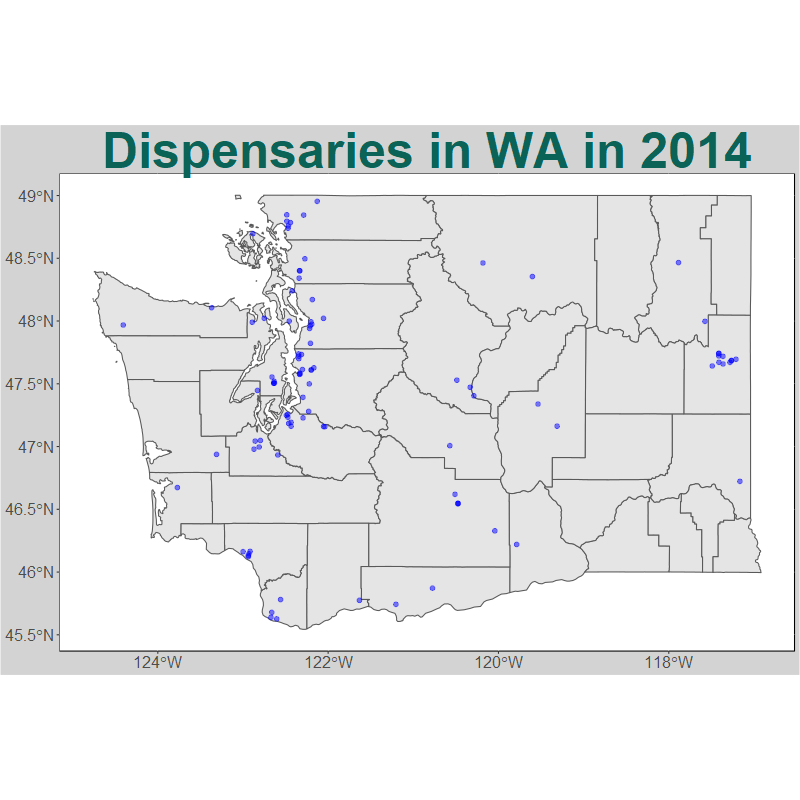
\includegraphics[width=.5\linewidth]{point_map_WA_2014.png}
	}
	\subfloat{
		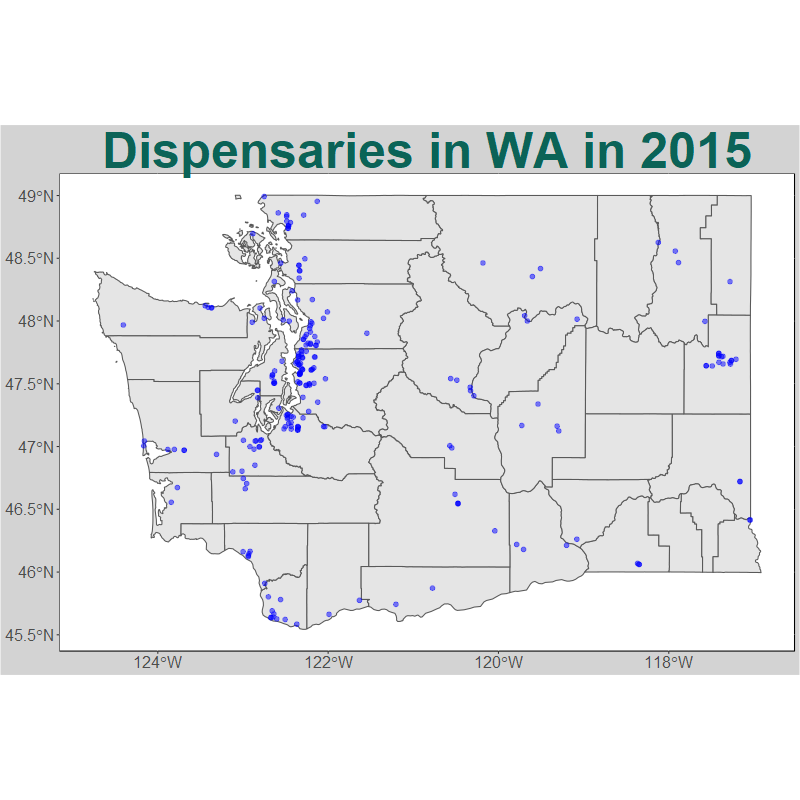
\includegraphics[width=.5\linewidth]{point_map_WA_2015.png}
	}
	\newline
	\subfloat{
		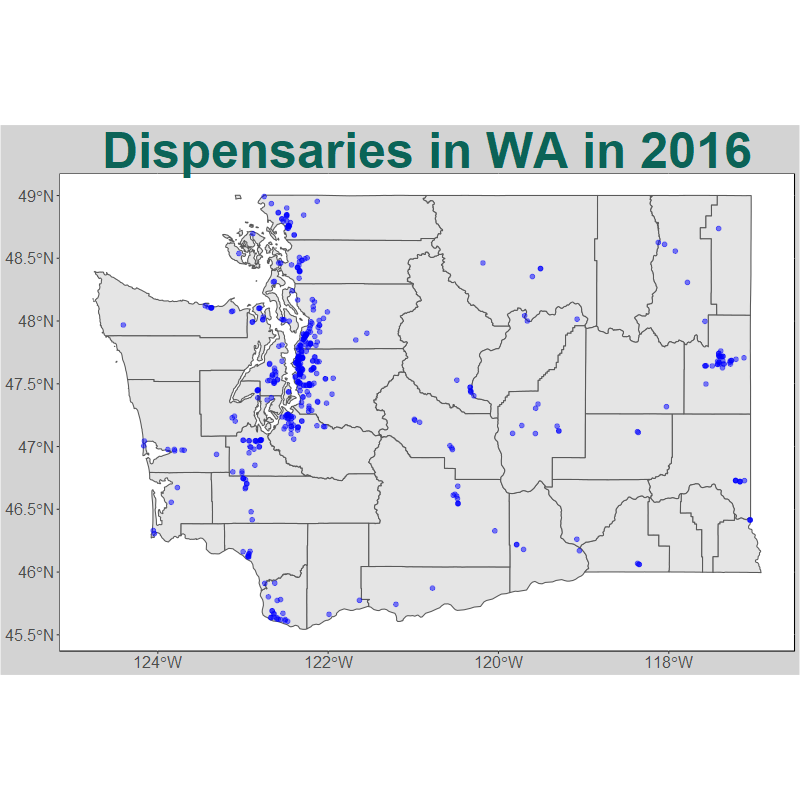
\includegraphics[width=.5\linewidth]{point_map_WA_2016.png}
	}
	-
\end{figure}



%------------------------------------------------------------------------------
% Empirical Analysis
%------------------------------------------------------------------------------

\section{Empirical Analysis}

\subsection{BRFSS Analysis}

My First approach to determine the effect of marijuana legalization on alcohol use is to use the BRFSS survey data along with indicators for changes in state laws. I estimate the following equation using a Tobit model. 

$$
ave\_drinks = \beta_0 +  \beta_1  rec\_l  + \beta_2MML + \bm{\beta_3 Year} + \bm{\beta_4 State} + \bm{\beta_5 Marital} + \bm{\beta_6 Edu} + \beta_7 Smoke
$$

\begin{center}
	\begin{tabular}{||c | c||} 
		\hline
		Variable & Meaning  \\ [0.5ex] 
		\hline\hline
		ave\_drinks & Average Drinks per Week \\ 
		\hline 
		rec\_l & Recreational Consumption is Legal in Respondent's State  \\ 
		\hline
		MML & Medical Marijuana is Legal in Respondent's State  \\
		\hline
		Year & Year Fixed Effects \\
		\hline
		State & State Fixed Effects\\
		\hline
		Marital & Marital Status Dummies  \\ 
		\hline
		Edu & Education level Dummies \\
		\hline
		Smoke & Have you smoked at least 100 cigarettes in your entire life\\[1ex] 
		\hline
	\end{tabular}
\end{center}


The Marital dummies include Married, Divorced, widowed, Separated, Never Married, Member of unmarried couple, refused. Education level is broken up into never attended kindergarten, grades 1-8, grades 9-11, high school graduate, some college or technical school, college graduate, or refused. The dummy for Recreational consumption being legal starts on the first day that laws in each state allowed personal consumption even if no legal dispensaries are open. \par 

I estimate a Tobit Model  \footnote{I considered using a hackmen selection model here instead, but it would not converge. I need to give this model a bit more thought but given the null results I focused more on the spatial analysis below.} because of censoring at Zero. Figure three Shows the distribution of respondents average drinks per week. 

\begin{center}
	
	\centering
	\textbf{Figure 3}\par\medskip
	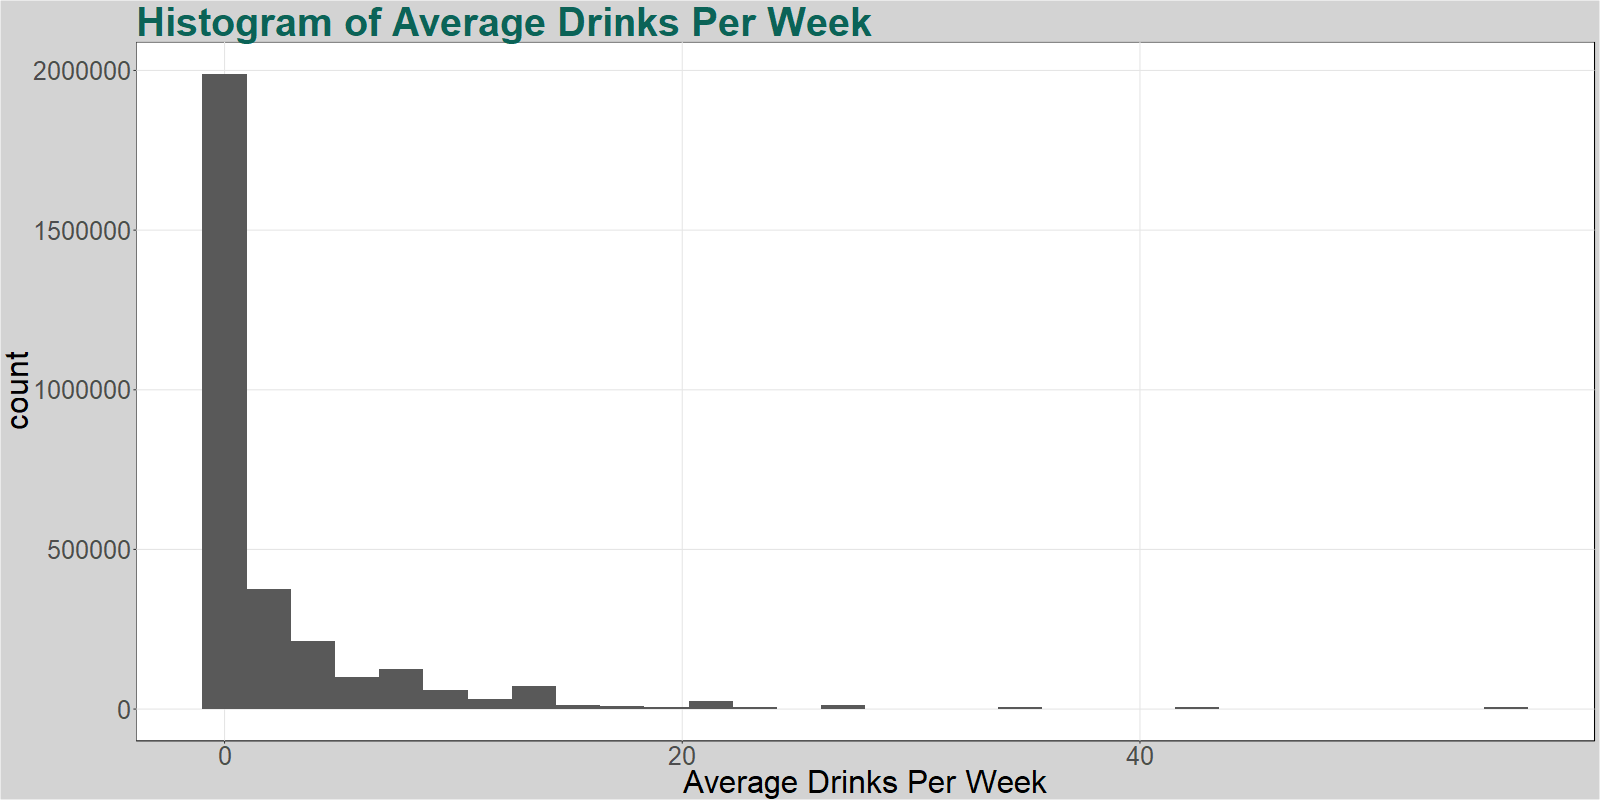
\includegraphics[width=1\linewidth]{Hist_nm_aved_week.png}
\end{center}

Admittedly, the interpretation of this as a Tobit model is a bit non standard. It's not entirely clear what the censored latent variable would be in this case since average weakly drinks is not actually capable of falling below zero. However, McDonald and Moffitt provide a decomposition and interpretation of the Tobit coefficients into "the effect on the probability of being above zero, and effects conditional upon being above zero" which justifies it's use \cite{Mcdon_moffit}. The coefficients of interest are reported in Table 1 below. 


\begin{center}
	
	\centering
		\LARGE{\textbf{Table 1}}\par\medskip
		
	\normalsize{\textbf{BRFSS Tobit Coefficient of Interest}}\par\medskip
	\scalebox{1}{
		\begin{tabular}{l*{1}{c}}
\hline\hline
            &\multicolumn{1}{c}{Average Drinks Per Week}\\
\hline
&            \\
Recreational Consumption is Legal in Respondent's State       &      0.0148\\
            &     (0.0495)\\
[1em]
Medical Marijuana is Legal in Respondent's State         &       -0.0147\\
            &     (0.0374)\\
\hline
\(N\)       &     3023271\\
\hline\hline
\end{tabular}

	}
\end{center}

The results for both coefficients are statistically insignificant. While I think the idea of using survey data is attractive the model design does not give us very much power. The only variation we can observe is at the state level. Furthermore, we can?t use the variation in access within the state because the data only reports the respondents state. This let gives us motivation for turning to the Nielsen scanner data.  The assumptions here are pretty strong, and we are still getting null results. It suggests to me that we need a measure with less measurement error and also more variation. Finer geographic data will provide this and directly measure sales is more precise even it is less accurately measures overall consumption. 


\subsection{Nielson Scanner analysis}

\begin{center}
	
	\centering
	
	\textbf{Nielson Scanner Regressions }\par\medskip
	\scalebox{.8}{
		% latex table generated in R 3.5.1 by xtable 1.8-3 package
% Mon Dec 17 10:42:49 2018
\begin{tabular}{lllllllll}
  \hline
Term & M1 Est & M1 SE & M2 Est & M2 SE & M3 Est & M3 SE & M4 Est & M4 SE \\ 
  \hline
Marijuana Legal to Consume & 0.2289 & 0.0361 & 0.1808 & 0.0323 & 0.1537 & 0.0316 & 0.1412 & 0.0317 \\ 
  Number of Dispensaries & -0.0019 & 0.0014 & -0.0023 & 0.0012 & -0.0024 & 0.0011 & -0.0025 & 0.001 \\ 
  Dispensary Distance Metric & 0.2082 & 0.0465 &  &  &  &  &  &  \\ 
  Dispensary Distance Metric X Marijuana Legal to Consume & -0.2073 & 0.0461 &  &  &  &  &  &  \\ 
  Dispensary Distance Metric V2 &  &  & 0.1609 & 0.0367 &  &  &  &  \\ 
  Dispensary Distance Metric V2 X Marijuana Legal to Consume &  &  & -0.1612 & 0.0366 &  &  &  &  \\ 
  Dispensary Distance Metric V3 &  &  &  &  & 0.1467 & 0.0492 &  &  \\ 
  Dispensary Distance Metric V3 X Marijuana Legal to Consume &  &  &  &  & -0.1475 & 0.0492 &  &  \\ 
  Dispensary Distance Metric V4 &  &  &  &  &  &  & 0.0998 & 0.0698 \\ 
  Dispensary Distance Metric V4 X Marijuana Legal to Consume &  &  &  &  &  &  & -0.1007 & 0.0698 \\ 
  Year FE & Yes & Yes & Yes & Yes & Yes & Yes & Yes & Yes \\ 
  County FE & Yes & Yes & Yes & Yes & Yes & Yes & Yes & Yes \\ 
   \hline
\end{tabular}

	}
\end{center}





%------------------------------------------------------------------------------
% Future work and Conclusion
%------------------------------------------------------------------------------

\section{Future work and Conclusion }


%------------------------------------------------------------------------------
% bib
%------------------------------------------------------------------------------
\bibliographystyle{apacite}
\bibliography{References}


%------------------------------------------------------------------------------
% Appendix 
%------------------------------------------------------------------------------

\section{Appendix}

\subsection{Appendix A}

\begin{figure}[H]
	\centering
	\LARGE{\textbf{Counties in Scanner Panel Per Month}}\par\medskip
	\scalebox{.6}{
	% latex table generated in R 3.5.1 by xtable 1.8-3 package
% Mon Dec 17 02:10:42 2018
\begin{tabular}{llr}
  \hline
year & month & Number of Counties \\ 
  \hline
2011 & 01 & 1806 \\ 
  2011 & 02 & 1807 \\ 
  2011 & 03 & 1812 \\ 
  2011 & 04 & 1812 \\ 
  2011 & 05 & 1813 \\ 
  2011 & 06 & 1817 \\ 
  2011 & 07 & 1867 \\ 
  2011 & 08 & 1872 \\ 
  2011 & 09 & 1868 \\ 
  2011 & 10 & 1871 \\ 
  2011 & 11 & 1871 \\ 
  2011 & 12 & 1875 \\ 
  2012 & 01 & 1847 \\ 
  2012 & 02 & 1836 \\ 
  2012 & 03 & 1875 \\ 
  2012 & 04 & 1874 \\ 
  2012 & 05 & 1891 \\ 
  2012 & 06 & 1888 \\ 
  2012 & 07 & 1884 \\ 
  2012 & 08 & 1881 \\ 
  2012 & 09 & 1893 \\ 
  2012 & 10 & 1882 \\ 
  2012 & 11 & 1881 \\ 
  2012 & 12 & 1876 \\ 
  2013 & 01 & 1863 \\ 
  2013 & 02 & 1844 \\ 
  2013 & 03 & 1853 \\ 
  2013 & 04 & 1854 \\ 
  2013 & 05 & 1864 \\ 
  2013 & 06 & 1900 \\ 
  2013 & 07 & 1900 \\ 
  2013 & 08 & 1881 \\ 
  2013 & 09 & 1879 \\ 
  2013 & 10 & 1873 \\ 
   \hline
\end{tabular}

}
	\scalebox{.6}{
	% latex table generated in R 3.5.1 by xtable 1.8-3 package
% Mon Dec 17 02:10:42 2018
\begin{tabular}{llr}
  \hline
year & month & Number of Counties \\ 
  \hline
2013 & 11 & 1884 \\ 
  2013 & 12 & 1887 \\ 
  2014 & 01 & 1858 \\ 
  2014 & 02 & 1862 \\ 
  2014 & 03 & 1866 \\ 
  2014 & 04 & 1868 \\ 
  2014 & 05 & 1878 \\ 
  2014 & 06 & 1890 \\ 
  2014 & 08 & 1889 \\ 
  2014 & 09 & 1888 \\ 
  2014 & 10 & 1885 \\ 
  2014 & 11 & 1893 \\ 
  2014 & 12 & 1892 \\ 
  2015 & 01 & 1878 \\ 
  2015 & 02 & 1883 \\ 
  2015 & 03 & 1895 \\ 
  2015 & 04 & 1905 \\ 
  2015 & 05 & 1919 \\ 
  2015 & 06 & 1926 \\ 
  2015 & 07 & 1940 \\ 
  2015 & 08 & 1950 \\ 
  2015 & 09 & 1964 \\ 
  2015 & 10 & 1956 \\ 
  2015 & 11 & 1952 \\ 
  2015 & 12 & 1948 \\ 
  2016 & 01 & 1945 \\ 
  2016 & 02 & 1936 \\ 
  2016 & 03 & 1934 \\ 
  2016 & 04 & 1941 \\ 
  2016 & 05 & 1939 \\ 
  2016 & 06 & 1944 \\ 
  2016 & 07 & 1947 \\ 
  2016 & 08 & 1946 \\ 
   \hline
\end{tabular}

}
\end{figure}


%------------------------------------------------
% end doc
%------------------------------------------------
\end{document}